\documentclass[../Head/Main.tex]{subfiles}
\begin{document}
\subsection{Q-learning}
Q-learning was implemented by designing a set of key methods.
\begin{itemize}
	\item[-] \texttt{getNextState(qState s, float a)} \vspace{-5pt}
	\item[-] \texttt{qUpdate(qState s, float $\alpha$, float $\gamma$, float $\epsilon$)} \vspace{-5pt}
	\item[-] \texttt{visitRoom(qState s)} \vspace{-5pt}
	\item[-] \texttt{getNextAction(qState s)} \vspace{-5pt}
	\item[-] \texttt{findStateMatrixIndex(qState s)} \vspace{-5pt} 
	\item[-] \texttt{findQMatrixIndex(qState s)} \vspace{-5pt}
	\item[-] \texttt{setDistancePunishment(qState s1, qState s2, float p)} \vspace{-5pt}
	\item[-] \texttt{setReward(int roomNumb, float reward)}
\end{itemize}


All these methods was implemented in a class called \texttt{q\_learning}. This gives the possibility of initialising all matrices and parameters in the constructor, only given the number of rooms as argument. This makes code scalable to any number of rooms.\\

\clearpage
It has been chosen to initialise all rewards to $-100$ except those on the main diagonal, whose initial value was set to $0$.\\
Calling the methods \texttt{setDistancePunishment(s1, s2, p)}, and \texttt{setReward(roomNumb, reward)} afterwards would update the total reward .\\
An example of how that would look like can be seen in table (\ref{tab:reward_matrix_5_room}), where all distance punishments are based on those found in the test in appendix (\ref{subsec:probability_test}) multiplied by a factor of $1.2$. The rewards for entering a room was found in the test in appendix (\ref{subsec:est_path_length}), and divided by the max value and then multiplied with a factor of 20. The initial room was set to 3 in this example.
\begin{table}[H]
	\centering
	\subfile{../Tables/q_learn_reward_matrix}
	\caption{Rewards for all state-action combinations given that no rooms have been visited and initial state is room 3}
	\vspace{-20pt}
	\label{tab:reward_matrix_5_room}
\end{table}
The vector \texttt{stateMatrix} contains the rewards, and it was chosen to keep this matrix dynamic, so only the combinations needed was added to the vector instead of all possible combinations, unlike the vector that contains the \texttt{qMatrix}. This was done because it makes no difference whether the state matrix only applies for one episode or all combinations, as long as the matrix is reset each time a new episode starts. Doing this saves memory.\par  
The method \texttt{setDistancePunishment(qState s1, qState s2, float p)} inserts a distance punishment between two states, by indexing the matrix with the room numbers of the two states. The indices are then reversed to apply the punishment in both directions.\par  

The method \texttt{visitRoom(qState s)} are one of the primary methods behind the mapping between the different layers in the Q-matrix. This method updates the vector in states by changing the value to true for the current room.\\
Then it is checked whether the state is terminal or not and updates this information in the state.\\
If the room does not appear in the list of visited rooms, it is then added and a new reward matrix will be generated based on the new states. The new state is then returned from the method.\par 

The method \texttt{findStateMatrixIndex(qState s)} is used to find the index for the \texttt{stateMatrix} containing all the rewards. The method works by comparing the values in the vector from the state with the values corresponding to the order in the state matrix. When a match is found, the corresponding index will be returned.\\
Due to the fact that is was chosen to make the \texttt{stateMatrix} dynamic, a second version of this method was written to find the index for the \texttt{qMatrix}. This method was called \texttt{findQMatrixIndex(qState s)}.\par 

The method \texttt{getNextState(qState s, float a)} returns the next state, given the current state and action. This simple method replaces the room number with action (new room) and returns the state.\par 

To get good performance and good results a series of tests were conducted to find good values of $\alpha$, $\gamma$ and $\epsilon$. All the following tests were made using the world 5-room world, which can be seen on figure (\ref{fig:5-room_world_impl}).
\begin{figure}[H]
	\centering
	\subfile{../Figures/Map_5_rooms}
	\caption{Illustration of the world 5-room world used for the test on Q-learning}
	\label{fig:5-room_world_impl}
\end{figure}
The first test conducted was to show the influence of $\epsilon$ and chose an appropriate value for future tests. This test can be seen in appendix (\ref{subsec:test_epsilon}).\\
In figure (\ref{fig:q-learn_epsilon_impl}) the results from the test can be seen. It can be seen that there is a clear connection between the value of $\epsilon$ and the performance of the Q-learning algorithm. The higher the value of $\epsilon$ is the more random the agent acts and more lower is the average reward after a given number of episodes. The average number of iterations per episode falls drastically with increasingly larger value of $\epsilon$. Based on the test, the best value of $\epsilon$ was chosen to be 0.05, due to the fact that this value gives a good average reward while taking fewer iterations, than the slightly better performing ($\epsilon=0.01$). 
\begin{figure}[H]
	\centering
	\begin{subfigure}[b]{0.49\textwidth}
		\centering
		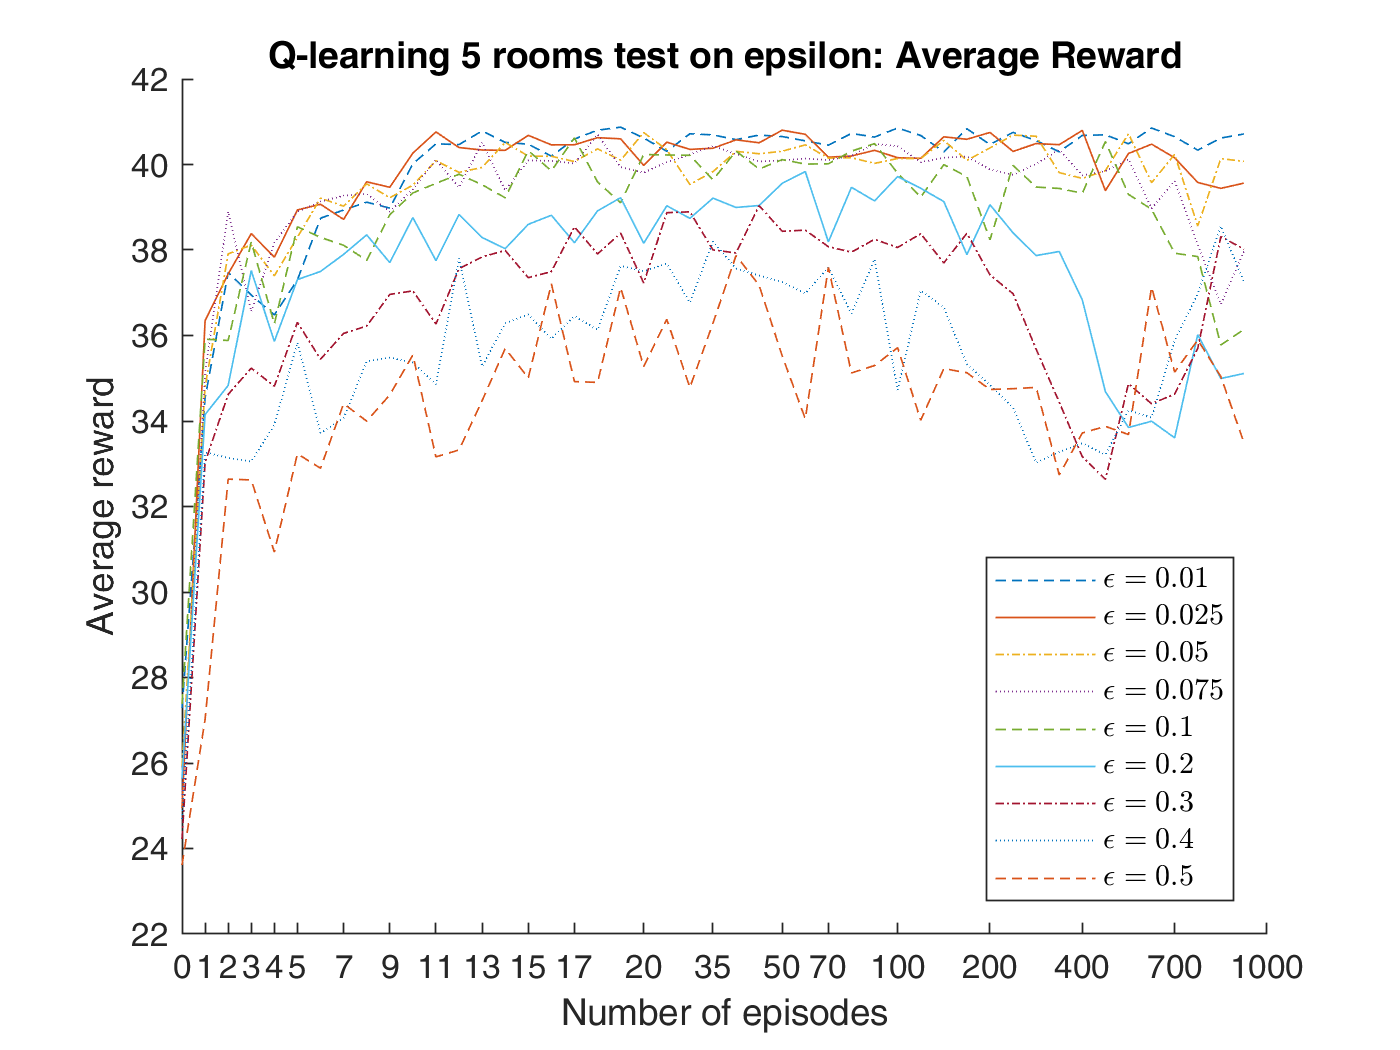
\includegraphics[width=\textwidth]{MatlabPlots/q_learning_5_rooms_test_epsilon_average_reward}
		\caption{Plot of how the average reward develops as a function of the number of episodes for each value of $\epsilon$}
		\label{fig:q-learn_epsilon_reward_impl}
	\end{subfigure}
	\hfill
	\begin{subfigure}[b]{0.49\textwidth}
		\centering
		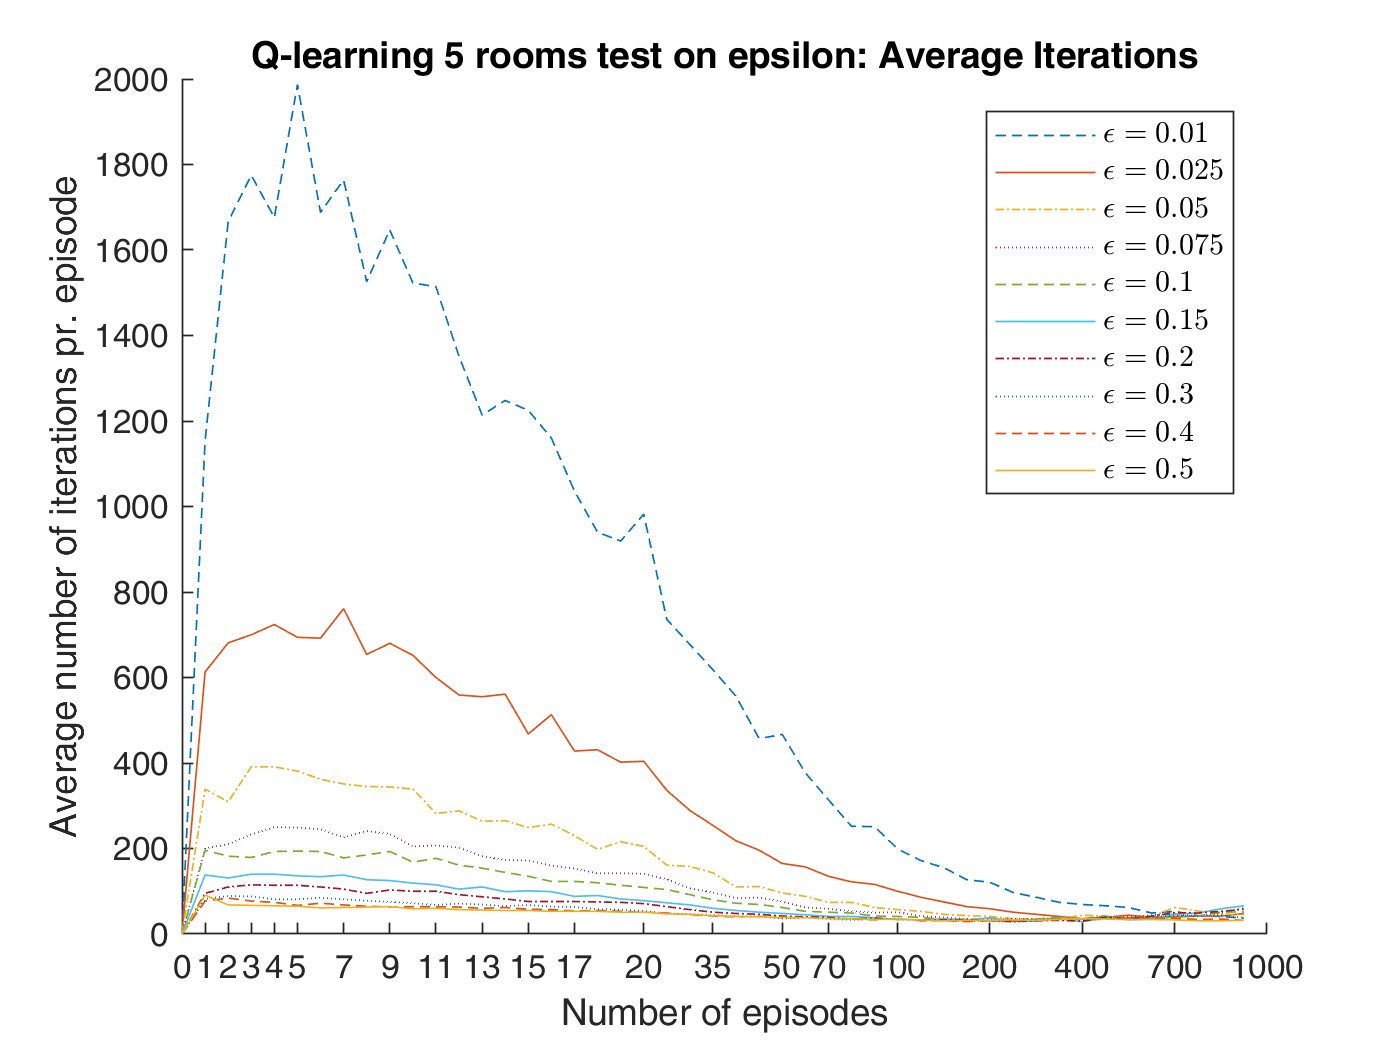
\includegraphics[width=\textwidth]{MatlabPlots/q_learning_5_rooms_test_epsilon_average_iterations}
		\caption{Plot of how the average number of episodes develops as a function of the number of episodes for each value of $\epsilon$}
		\label{fig:q-learn_epsilon_iterations_impl}
	\end{subfigure}
	\caption{Plots of both the average reward and average number of iterations pr. episode for each value of $\epsilon$}
	\label{fig:q-learn_epsilon_impl}
\end{figure}
The next test conducted was to show the influence of the learning rate $\alpha$. The test can be seen in appendix (\ref{subsec:test_alpha}).\\
In figure (\ref{fig:q-learn_alpha_impl}) the result from the test can be seen. From the test results it can be seen that with a decreasing learning rate the average reward increases and the longer the number of iterations keeps high. This means that the lower the learning rate the longer it will take to learn, but what it have learnt would be more optimal than with higher values of $\alpha$. Based on the test  a value of $\alpha$ was chosen to be 0.025.
\begin{figure}[H]
	\centering
	\begin{subfigure}[b]{0.49\textwidth}
		\centering
		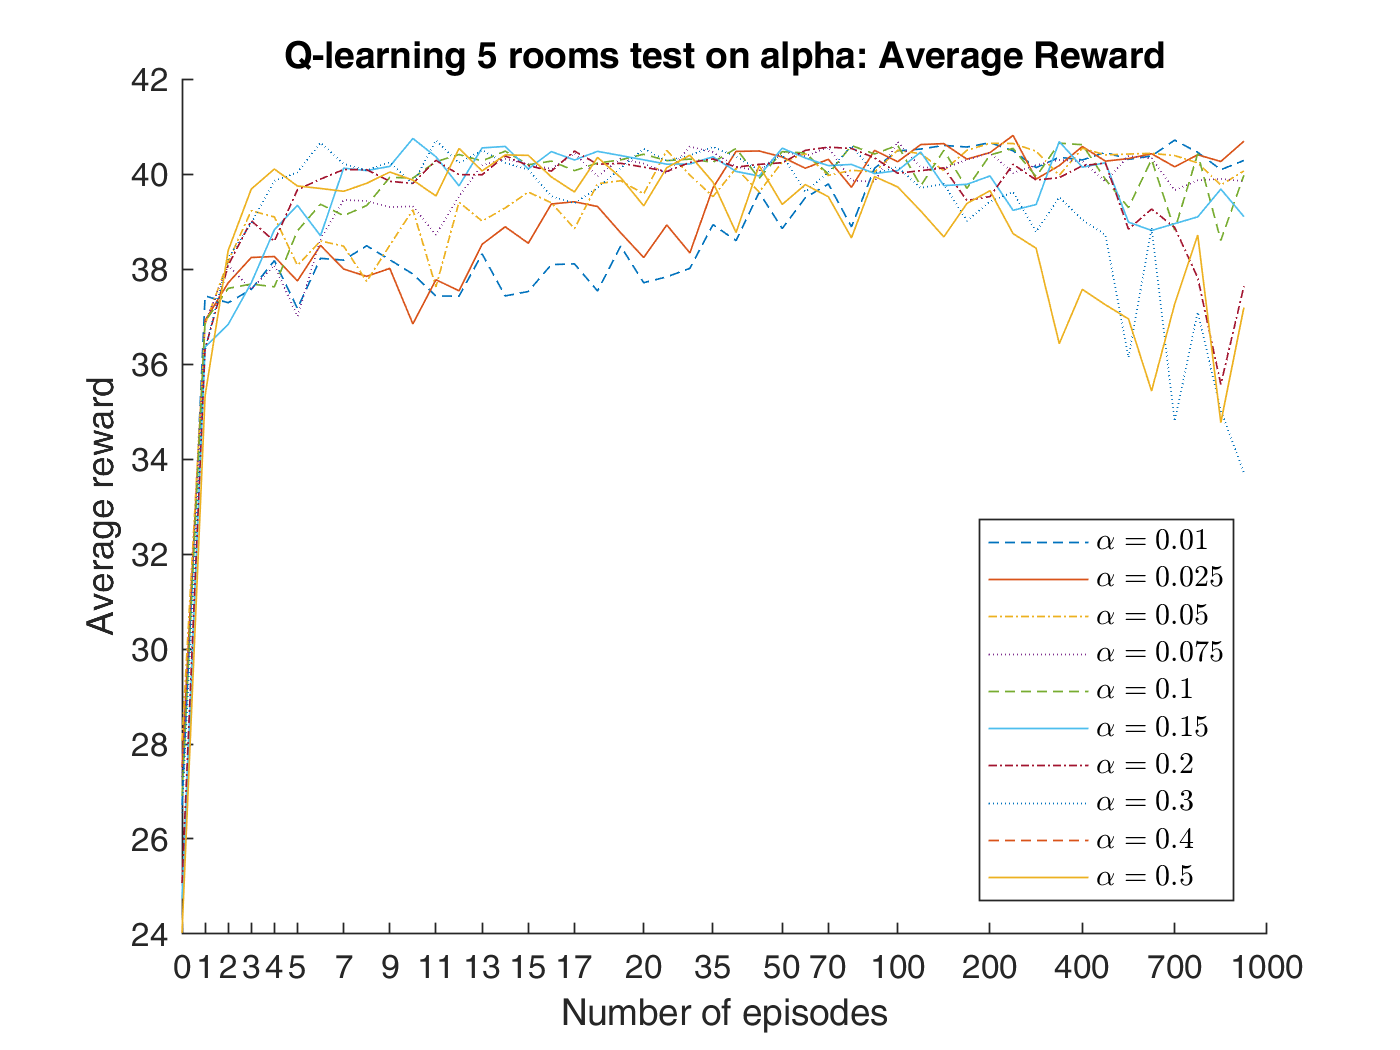
\includegraphics[width=\textwidth]{MatlabPlots/q_learning_5_rooms_test_alpha_average_reward}
		\caption{Plot of how the average reward develops as a function of the number of episodes for each value of $\epsilon$}
		\label{fig:q-learn_alpha_reward_impl}
	\end{subfigure}
	\hfill
	\begin{subfigure}[b]{0.49\textwidth}
		\centering
		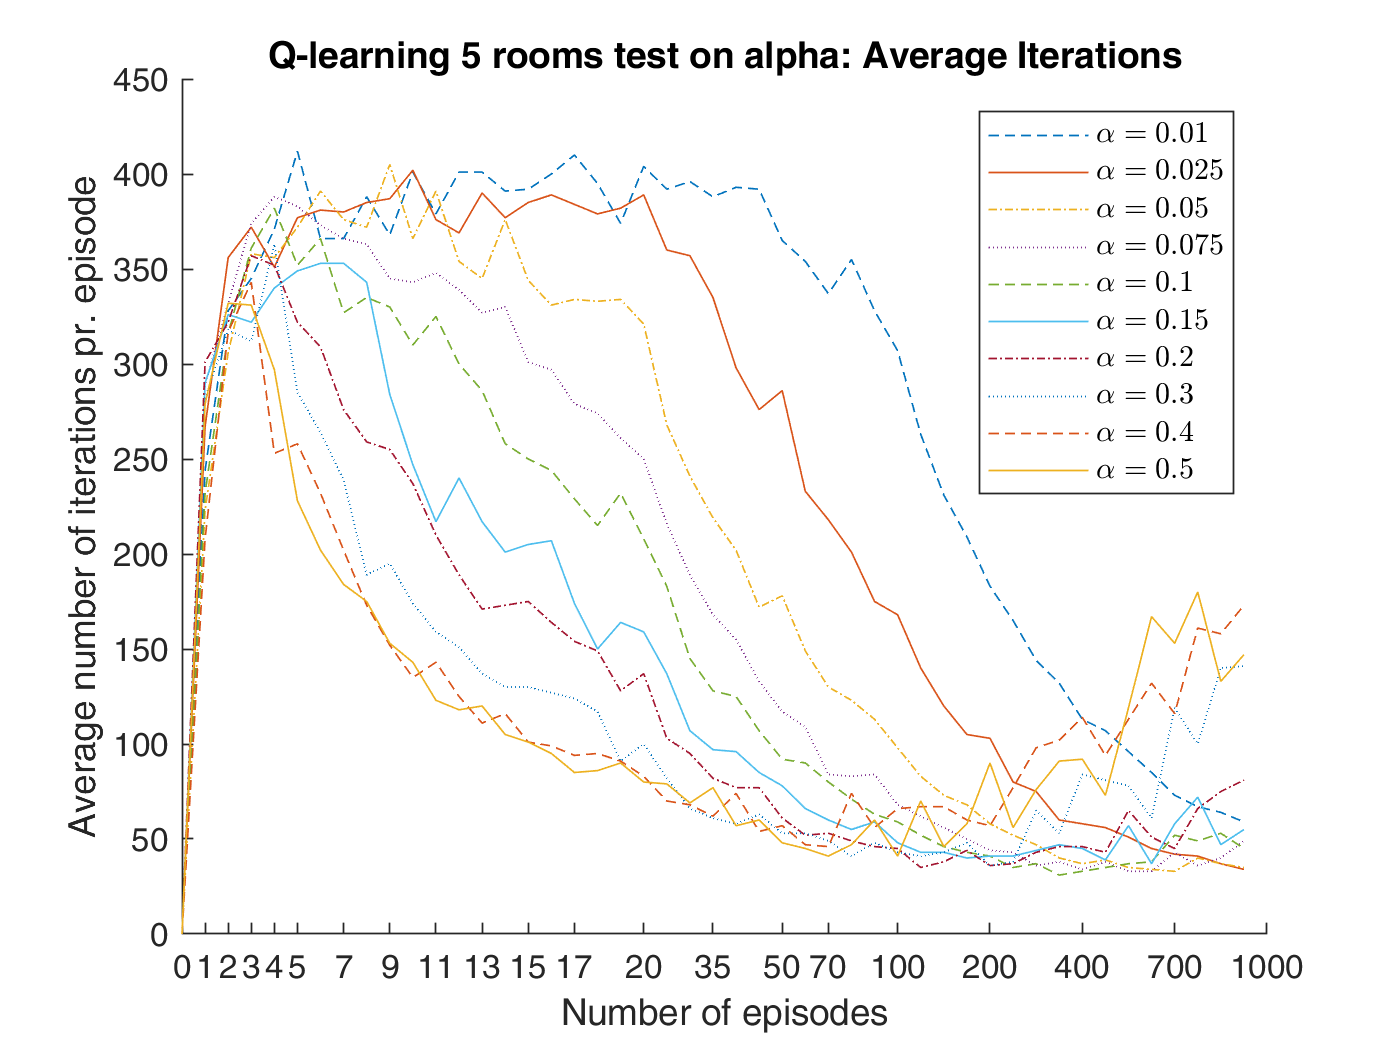
\includegraphics[width=\textwidth]{MatlabPlots/q_learning_5_rooms_test_alpha_average_iterations}
		\caption{Plot of how the average number of episodes develops as a function of the number of episodes for each value of $\alpha$}
		\label{fig:q-learn_alpha_iterations_impl}
	\end{subfigure}
	\caption{Plots of both the average reward and average number of iterations pr. episode for each value of $\alpha$}
	\label{fig:q-learn_alpha_impl}
\end{figure}

\clearpage
The final parameter was tested in the following test. The purpose of this test was to show the influence of the discount factor $\gamma$. This test can be seen in appendix (\ref{subsec:test_gamma}). In figure (\ref{fig:q-learn_gamma_impl}) the results from the test can be seen. From the results it can be seen that the higher the value of $\gamma$ the fewer iterations are needed to perform an episode, and the less varying the average reward will be. Given the test a value of $\gamma$ was chosen to be 0.99.

\begin{figure}[H]
	\centering
	\begin{subfigure}[b]{0.49\textwidth}
		\centering
		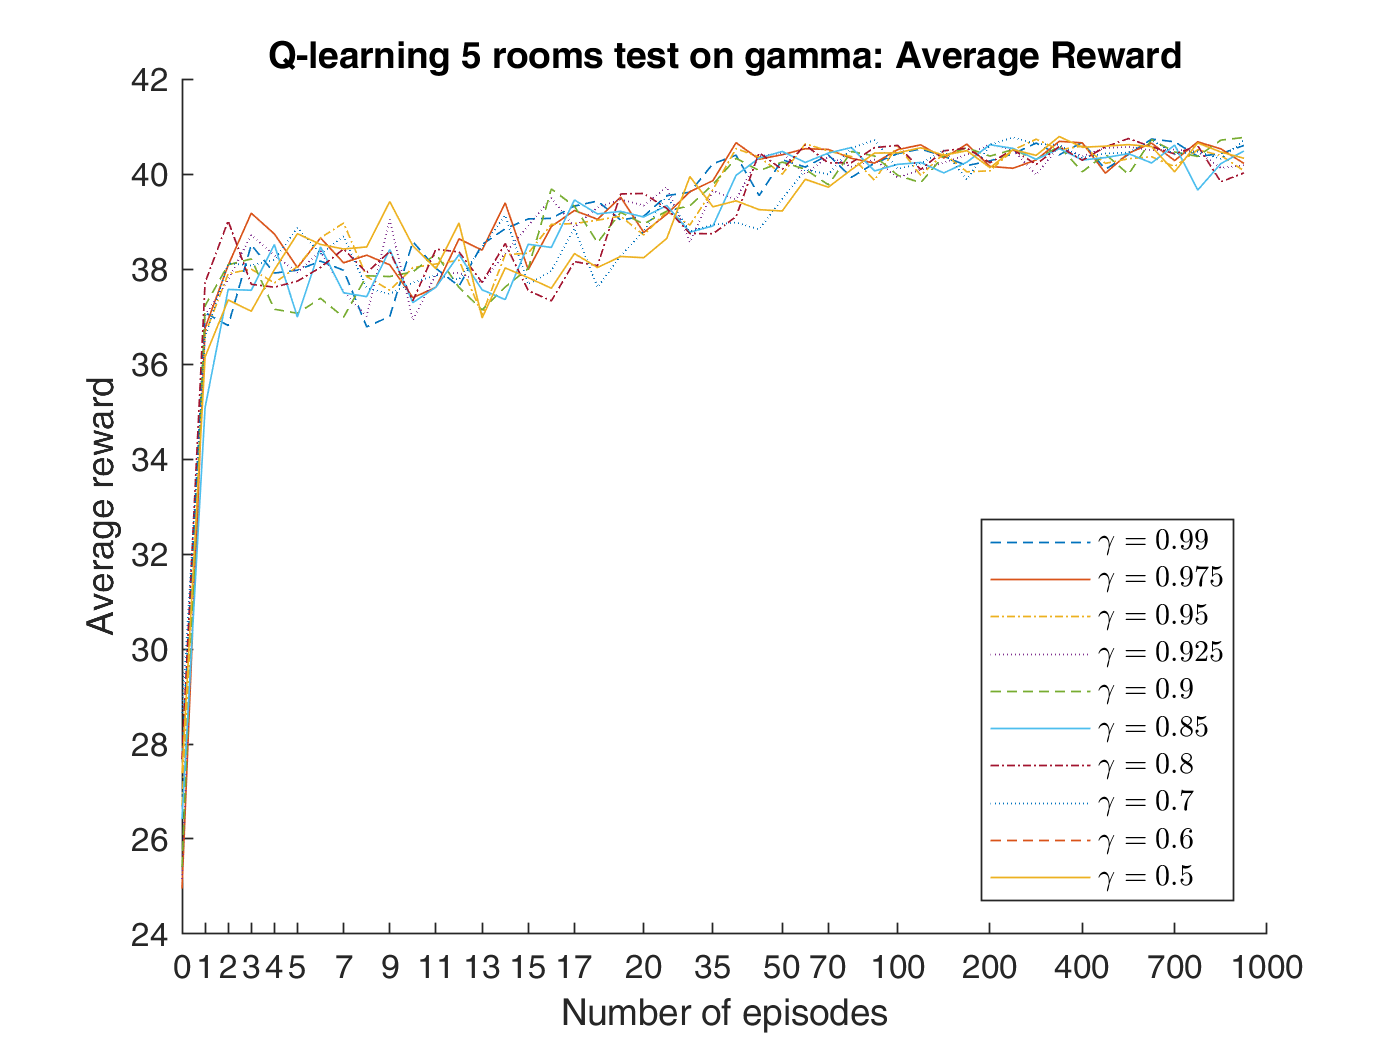
\includegraphics[width=\textwidth]{MatlabPlots/q_learning_5_rooms_test_gamma_average_reward}
		\caption{Plot of how the average reward develops as a function of the number of episodes for each value of $\epsilon$}
		\label{fig:q-learn_gamma_reward_impl}
	\end{subfigure}
	\hfill
	\begin{subfigure}[b]{0.49\textwidth}
		\centering
		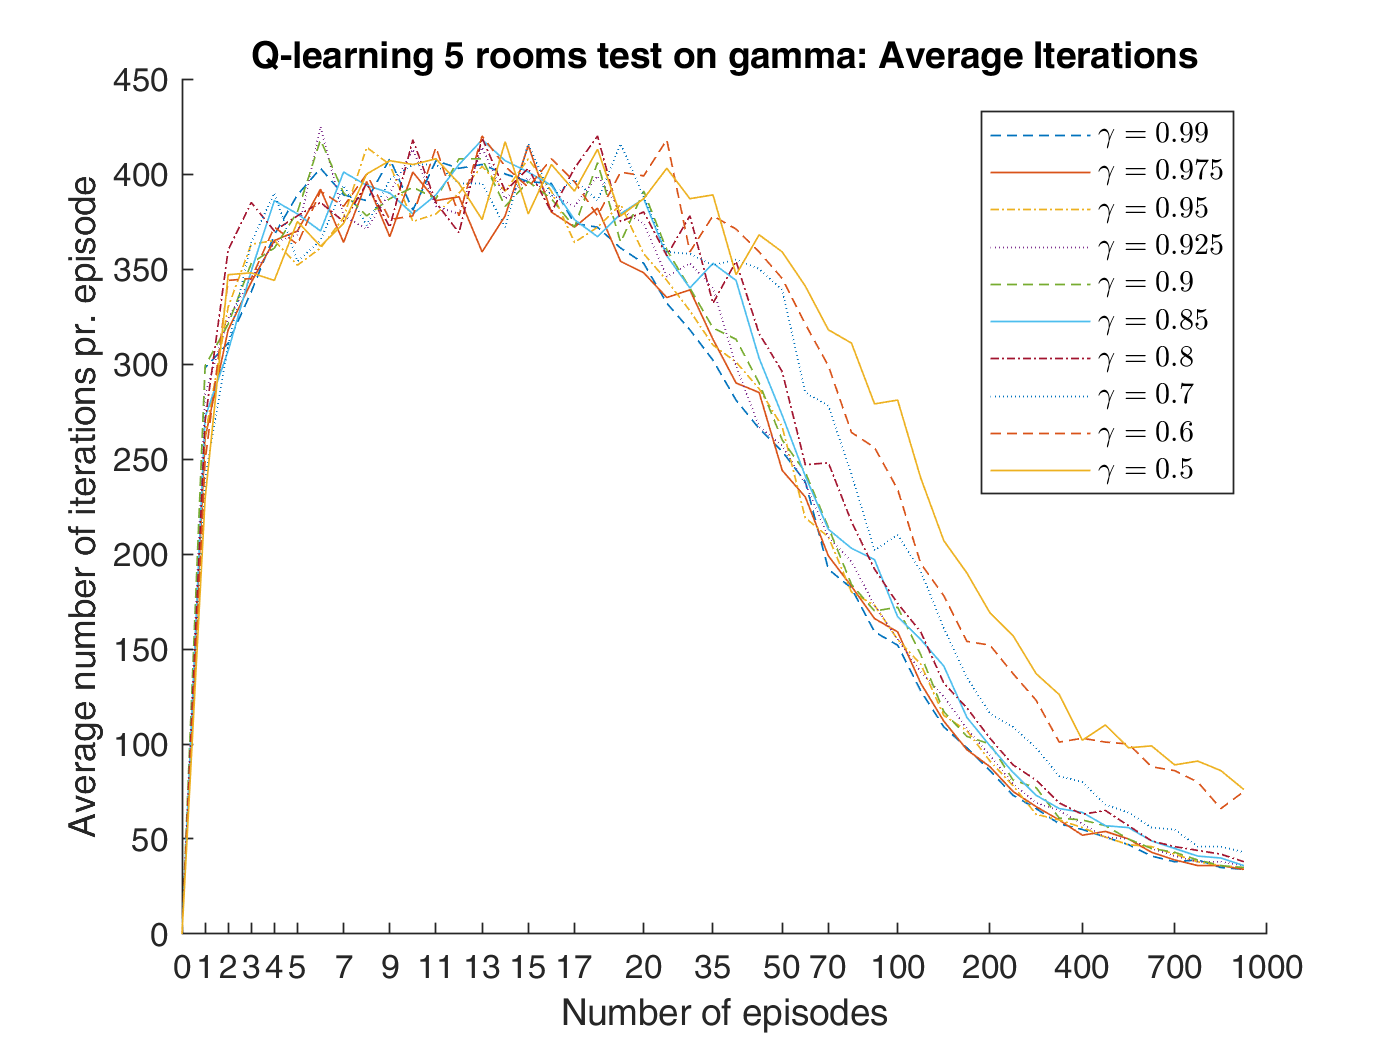
\includegraphics[width=\textwidth]{MatlabPlots/q_learning_5_rooms_test_gamma_average_iterations}
		\caption{Plot of how the average number of episodes develops as a function of the number of episodes for each value of $\alpha$}
		\label{fig:q-learn_gamma_iterations_impl}
	\end{subfigure}
	\caption{Plots of both the average reward and average number of iterations pr. episode for each value of $\gamma$}
	\label{fig:q-learn_gamma_impl}
\end{figure}
Based on those three test, a good set-up was found for the final test on getting a good path. It has also been chosen to conduct a test on finding an optimal path on the 5-room world. This test can be seen in appendix (\ref{subsec:test_best_path}). In this test, the parameters used were found in the previous tests. A total of 5 subtest were made in order to find an optimal path for navigating the 5-room world. The agent was started in all rooms, and had to learn its way through the environment. The agent was given 2000 episodes to learn, before returning the learnt path. This was done ten times for each room to get an idea of the average case. Based on this test, the best average case was when the agent started in room 1, but the best path was found with start in both room 1 and 5. These paths can be seen in table (\ref{tab:q_learn_result}).

\begin{table}[H]
	\centering
	\begin{tabular}{r l r}
	\hline
	\multicolumn{1}{l}{\textbf{Initial room}} & \textbf{Path} & \textbf{Reward} \\ 			\hline
	1  & 0, 1, 2, 3, 5, 3, 4  & 44.4681\\
	5  & 0, 5, 3, 4, 3, 2, 1  & 44.4681\\
	\hline
	\end{tabular}
	\caption{The two best paths through the 5-room world found using the \texttt{q\_learning} class}
	\label{tab:q_learn_result}
\end{table}
This test would be scalable to larger environments, but test on higher number of rooms was not conducted due to time constrains.
\end{document}